% 	    %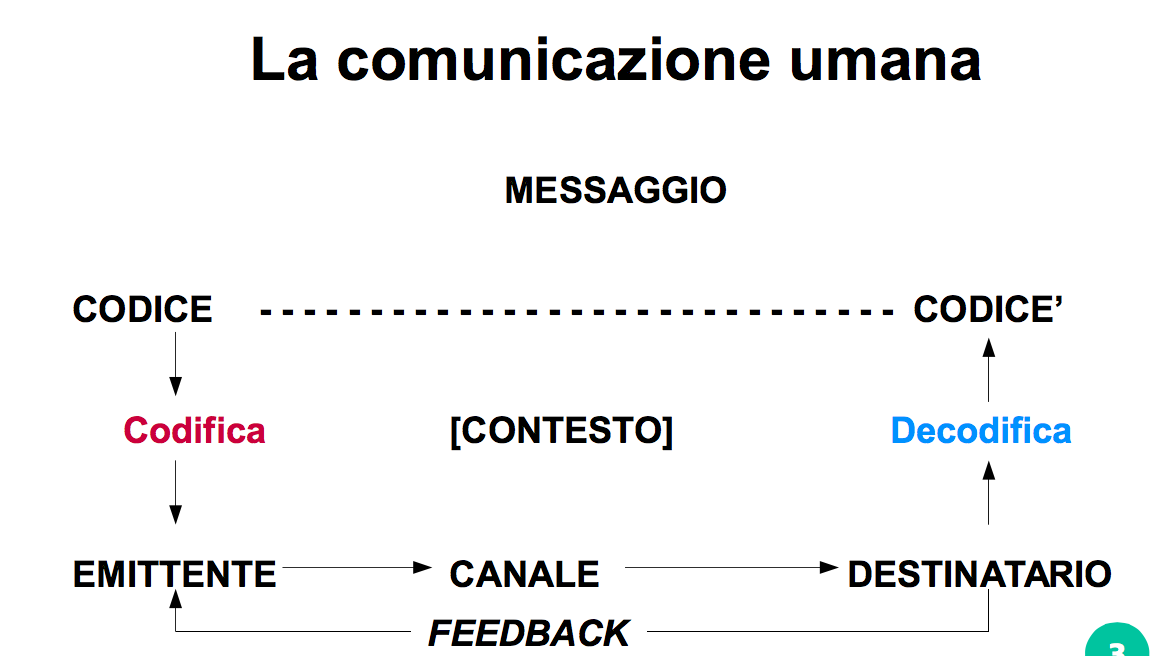
\includegraphics[width=.5\textwidth]{../imgs/comunicazioneUmana.png}
% definizione di segre
% definizione di tito orlandi

\begin{frame}
	\frametitle{Modellare il testo}
	\framesubtitle{Il testo come oggetto del dominio di studio}
	\addtocounter{nframe}{1}

	\begin{block}{Informatica nelle scienze umane}
		L'informatica umanistica ruota attorno alla rappresentazione e all'elaborazione degli oggetti che costituiscono il dominio delle discipline umanistiche.
	\end{block}

	\begin{block}{Testo come oggetto di studio}
		Il testo è, tra questi, l'oggetto più ricorrente
	\end{block}

\end{frame}

\begin{frame}
	\frametitle{Modellare il testo}
	\framesubtitle{qual è la natura del testo?}
	\addtocounter{nframe}{1}

	\begin{block}{Modellare il testo}
		Per trattare e rappresentare il testo in ambiente digitale, bisogna formulare un suo modello
	\end{block}

	\begin{block}{Modello del testo}
		Un efficace modello del testo non può prescindere da una determinazione di cosa si intenda per testo e la sua natura. Il fatto è che la rappresentazione (e a maggior ragione l’elaborazione) informatica è ontologicamente formale in senso stretto (Ciotti).
	\end{block}

\end{frame}

\begin{frame}
	\frametitle{Modellare il testo}
	\framesubtitle{Testo: oggetto complesso}
	\addtocounter{nframe}{1}

	\begin{block}{Cos'è il testo}
		Il testo è un oggetto complesso in quanto è in grado di veicolare significato su più livelli strutturali (logico, ontologico, linguistico, autoriale, editoriale, fisico, ecc.), anche attraverso l’instaurazione di molteplici relazioni tra più livelli.
	\end{block}

	\begin{block}{Cos'è il testo}
		Si tratta di una entità informativa complessa in quanto è il prodotto di più agenti e più fattori
	\end{block}

\end{frame}

\begin{frame}
	\frametitle{Modellare il testo}
	\framesubtitle{Testo: oggetto complesso}
	\addtocounter{nframe}{1}

	\begin{block}{Ma..}
		Non possediamo nessuna teoria sufficientemente completa del testo
	\end{block}

\end{frame}

\begin{frame}
	\frametitle{Modellare il testo}
	\framesubtitle{Tentativo..}
	\addtocounter{nframe}{1}

	\begin{block}{Cos'è il testo}
		Quale concezione o modello ontologico del testo è implicata nella rappresentazione informatica di esso?
	\end{block}

	\begin{block}{A quali teorie possiamo rivolgerci?}
		Molteplici teorie del testo, quasi tutte sbilanciate sul livello verbale-semantico (linguistica testuale).
	\end{block}

\end{frame}

\begin{frame}
	\frametitle{Modellare il testo}
	\framesubtitle{Tentativo..}
	\addtocounter{nframe}{1}

	\begin{block}{Cos'è il testo}
		Il termine ``testo''  si riferisce a un oggetto plurale, in cui co-esistono:
		\begin{itemize}
			\item Un livello astratto: la sequenza verbale, la quale a sua volta genera una serie di livelli di contenuti semantici.
			\item Un livello materiale: il supporto e le tracce d’inchiostro.
			\item Un livello dinamico: il testo viene creato da un autore e ricreato dal lettore.
		\end{itemize}

	\end{block}

\end{frame}


\begin{frame}
	\frametitle{Modellare il testo}
	\framesubtitle{Il testo: Cercando una definizione}
	\addtocounter{nframe}{1}

	\begin{block}{Cos'è il testo}
		\begin{itemize}
			\item Un documento materiale composto da fogli che contengono inchiostro variamente disposti?
			\item Un discorso linguistico fissato tramite la scrittura su un documento materiale?
			\item Un’opera dell’ingegno che viene costituita e fissata tramite un insieme di simboli/segni?
			\item Il contenuto di un messaggio?
		\end{itemize}
	\end{block}
\end{frame}

\begin{frame}
	\frametitle{Modellare il testo}
	\framesubtitle{Il testo: Cercando una definizione}
	\addtocounter{nframe}{1}

	\begin{block}{Cos'è il testo - uno sguardo più specialistico}
		\begin{itemize}
			\item Lo stato linguistico di un singolo testimone materiale di un’opera?
			\item Lo stato linguistico di un medesimo testimone di un’opera che presenta diverse lezioni identificabili?
			\item Una versione edita di un’opera?
			\item Una sequenza coerente di enunciati in una lingua naturale?
			\item Uno scritto che può essere trasmesso anche oralmente?
		\end{itemize}
	\end{block}

\end{frame}

\begin{frame}
	\frametitle{Modellare il testo}
	\framesubtitle{Definizioni}
	\addtocounter{nframe}{1}

	\begin{block}{Il testo}
		Dal latino \textit{textum}, participio passato di texere ``tessere'' quindi un testo è un ``tessuto'', un ordito di unità di significato (\textbf{monemi}) veicolato da simboli (\textbf{grafemi}).
	\end{block}

\end{frame}

\begin{frame}
	\frametitle{Modellare il testo}
	\framesubtitle{Definizioni}
	\addtocounter{nframe}{1}

	\begin{block}{Il testo secondo Segre 1985}
		Il testo è dunque una successione fissa di significati grafici. Questi significati sono poi portatori di significati semantici.
	\end{block}

\end{frame}

\begin{frame}
	\frametitle{Modellare il testo}
	\framesubtitle{Definizioni}
	\addtocounter{nframe}{1}

	\begin{block}{Il testo secondo Tito Orlandi 2010}
		La produzione di un'attività linguistica intesa in senso stretto, cioè in una delle lingue storicamente date, secondo il concetto saussuriano di \textit{langue} che produce la \textit{parole}. Il fatto che essa sia finalizzata a trasmettere un messaggio, pur importante in sé, non interessa per il momento se non marginalmente.
	\end{block}

\end{frame}


\begin{frame}
	\frametitle{Modellare il testo}
	\framesubtitle{Definizioni}
	\addtocounter{nframe}{1}

	\begin{block}{Ancora Tito Orlandi}
		Il Testo si presenta al lettore sotto la forma di rappresentazione di un'espressione linguistica, e poiché l'attività linguistica è multiforme, potrà essere una rappresentazione puramente mentale, astratta, ovvero fonica (verbale), ovvero grafica (scrittura).
	\end{block}


\end{frame}


\begin{frame}
	\frametitle{Modellare il testo}
	\framesubtitle{Definizioni}
	\addtocounter{nframe}{1}

	\begin{center}
		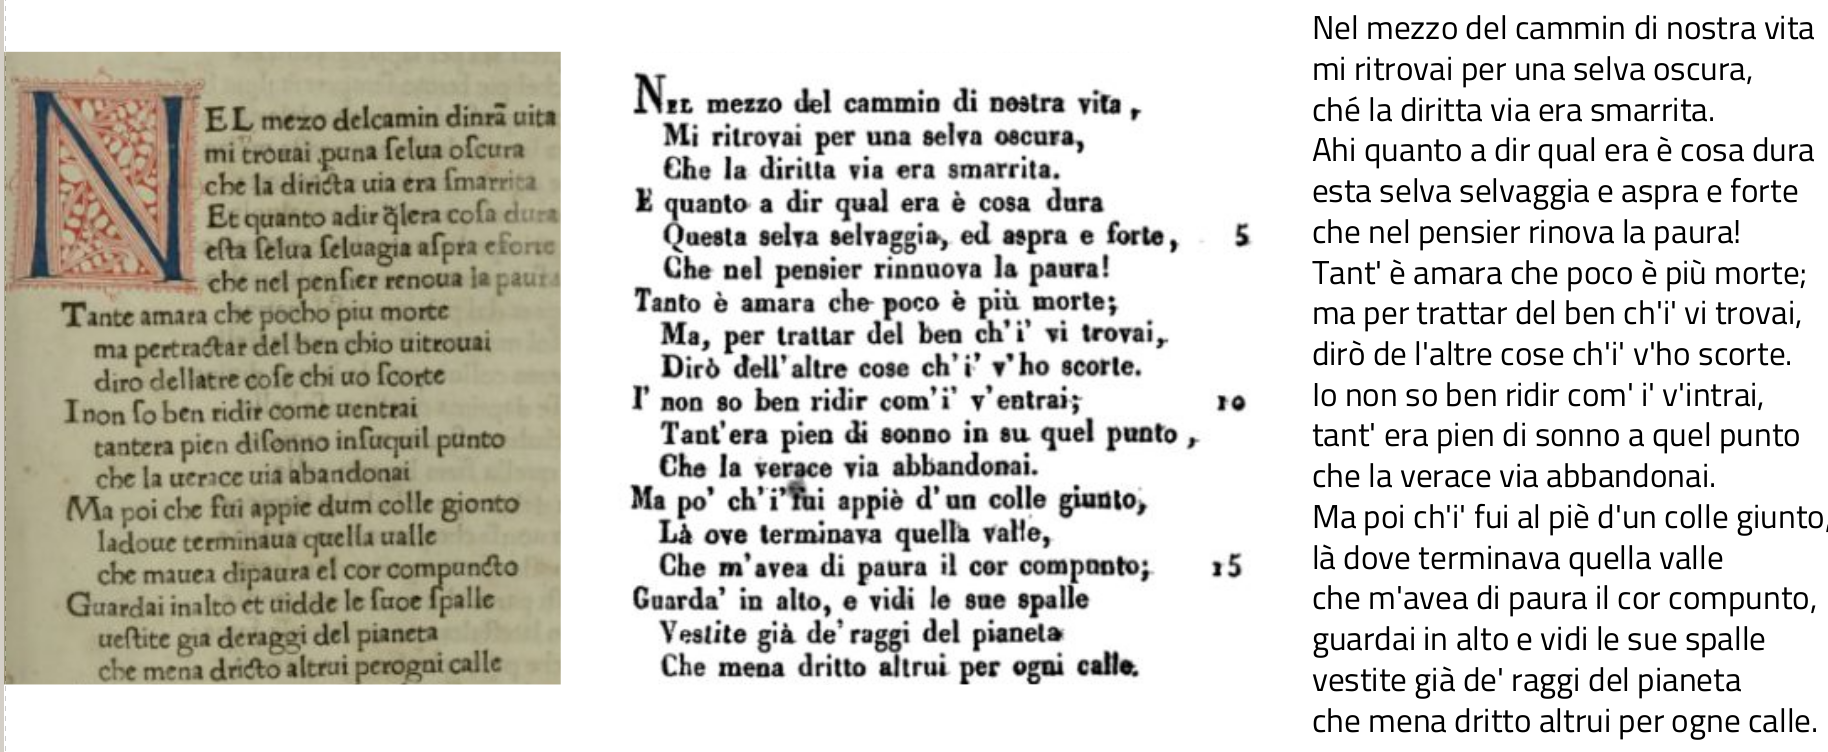
\includegraphics[width=.9\textwidth]{imgs/TestoDante.png}
	\end{center}

	\begin{block}{Possiamo concludere che}
		Il testo è l'invariante, la successione di valori, rispetto alle variabili dei caratteri, della scrittura.
	\end{block}

\end{frame}


% Teso è l'invariante rispetto ai segni, è la succesione di valori invariabili. Il testo, dunque è ciò che permane, l’invariante, in ogni operazione di riproduzione materiale della sequenza di simboli grafici.

% Questa definizione di testo come un oggetto astratto allografico sembra fornire un criterio di individuazione di un testo in base al principio di identità per sostituzione

\begin{frame}
	\frametitle{Modellare il testo}
	\framesubtitle{Complessità del testo}
	\addtocounter{nframe}{1}

	\begin{block}{Il testo oggetto complesso multidimensionale/pluralista}
		\begin{itemize}
			\item analisi grafematica (caratteri, ideogrammi)
			\item analisi strutturale (struttura editoriale, interna)
			\item analisi metrica (piedi, versi, stanze, strofe)
			\item analisi stilistica e retorica
			\item analisi tematica
			\item analisi semantica
			\item ecc..
		\end{itemize}
	\end{block}

\end{frame}

\begin{frame}
	\frametitle{Modellare il testo}
	\framesubtitle{Il testo letterario}
	\addtocounter{nframe}{1}

	\begin{block}{Particolarità del testo letterario}
		\begin{itemize}
			\item L'emittente prepara il messaggio, il destinatario potrebbe riceverlo anche dopo molto tempo
			\item Il feedback molto spesso non è possibile
			\item Il codice dell'emittente e quello del destinatario possono risultare diversi (o solo parzialmente compatibili)
		\end{itemize}
	\end{block}

\end{frame}


% Testo vs Documento


\begin{frame}
	\frametitle{Modellare il testo}
	\framesubtitle{Il documento}
	\addtocounter{nframe}{1}

	\begin{block}{Il Testo non è il Documento}
		La parola documento deriva dalla parola latina ``documentum'' che ha la stessa radice di ``doceo'' che significa ``insegnare''/``dimostrare'' con l'aggiunta del suffisso ``-umentum'' che intende lo strumento per fare.
	\end{block}

	\begin{block}{Il Documento}
		La parola ``documento'' designa quindi uno strumento per insegnare o uno strumento atto a dimostrare qualcosa.
	\end{block}


\end{frame}

\begin{frame}
	\frametitle{Modellare il testo}
	\framesubtitle{Il documento: Cercando una definizione}
	\addtocounter{nframe}{1}

	\begin{block}{Cos'è un documento}
		\begin{itemize}
			\item Una prova o una evidenza?
			\item Un atto cartaceo originale e/o ufficiale attraverso il quale dimostrare o provare qualcosa?
			\item Qualsiasi cosa materiale che serva come evidenza o prova?
			\item Un qualcosa di scritto contenente informazioni?
			\item Un supporto materiale sul quale sono stati rappresentati fatti o pensieri attraverso un qualche tipo di convenzione fatta di simboli e segni?
		\end{itemize}

	\end{block}

\end{frame}


%The first definition is more general. 
%The second one catches the most intuitive association of a document to a paper support, 
%while the third one extends the definition to all other kinds of support that may have the same function. 
%While all these definitions mainly focus on the bureaucratic, administrative or juridic aspects
%of documents, 
%the fourth and fifth ones are more interested in its role of information bearer that can be exploited for study, research information. 
%Again, the former covers the classical meaning of documents as written papers, while the latter extends it to any kind of support and representation. 
%Summing up, three aspects can be considered as relevant in identifying a document: its original meaning is captured
%by definitions 4 and 5, while definition 1 extends it to underline its importance as a proof of something, and definitions 2 and 3 in some way formally recognize this role in the social establishment.

\begin{frame}
	\frametitle{Modellare il testo}
	\framesubtitle{Definizioni}
	\addtocounter{nframe}{1}

	\begin{block}{Testo}
		Il testo è una entità astratta invariante, che in ogni operazione di realizzazione materiale della sequenza di simboli grafici determina la struttura fisica di un oggetto sensibilmente concreto (ovvero capace di attivare uno dei canali recettivi dell’uomo verso stimoli esterni).
	\end{block}

	\begin{block}{Documento}
		L'oggetto materiale, sensibile, concreto che costituisce il supporto, stabile e riproducibile dell’informazione testuale che determina una modalità d’interazione (lettura, decifrazione).
	\end{block}

\end{frame}

\begin{frame}
	\frametitle{Modellare il testo}
	\framesubtitle{Codifica del documento}
	\addtocounter{nframe}{1}

	\begin{block}{Il testo non è il documento}
		La codifica di un documento è diversa dalla codifica di un
		testo \textbf{(testo != documento)}. Si può parlare di documenti cartacei e di documenti
		digitali, ma non di testi cartacei e testi digitali!
	\end{block}

	\begin{block}{Documento digitale}
		Corrispondenza perfetta con l'originale: documento digitale
	\end{block}


\end{frame}

\begin{frame}
	\frametitle{Modellare il testo}
	\framesubtitle{Struttura del testo}
	\addtocounter{nframe}{1}

	\begin{block}{Elementi di un testo}
		Oltre alla sequenza di grafemi, un testo si presenta strutturato in segmentazioni logiche e partizioni interne di interi blocchi
	\end{block}

	\begin{block}{Struttura di un testo}
		Il testo ha una certa struttura, i cui elementi sono determinati dalla struttura logico-semantica del discorso con finalità e funzioni ben distinte (titolo di un capitolo, corpo di un paragrafo)
	\end{block}

\end{frame}

% esiste anche un modello documento
\begin{frame}
	\frametitle{Modellare il testo}
	\framesubtitle{Struttura del documento}
	\addtocounter{nframe}{1}

	\begin{block}{Struttura di un documento}
		Un documento, ugualmente, è costituito da elementi significativi, non solo verbali, da esplicitare formalmente (layout, segmentazione, foliazione, aspetti paratestuali, aspetti tipografici, aspetti topografici).
		% tipografica: Della tipografia, che ha relazione con la tipografia, cioè con la stampa
		%topografica: dislocazione o posizione reciproca dei varî elementi o delle varie parti che concorrono a formarlo
	\end{block}

\end{frame}




\begin{frame}
	\frametitle{Modellare il testo}
	\framesubtitle{Modelli concettuali}
	\addtocounter{nframe}{1}

	\begin{block}{Il testo è strutturato}
		Il testo è un oggetto reale dotato di una sua struttura che corrisponde alla struttura del linguaggio di rappresentazione;
	\end{block}

	\begin{block}{La natura del testo come OHCO}
		In un famoso articolo (DeRose et al., 1990) gli autori tentarono di dimostrare che il testo è una ``ordered hierarchy of content objects (OHCO)'': una gerarchia ordinata di oggetti di contenuto.
	\end{block}
\end{frame}


\begin{frame}
	\frametitle{Modellare il testo}
	\framesubtitle{Ordered Hierarchy of Content Objects (OHCO)}
	\addtocounter{nframe}{1}

	\begin{block}{La natura del testo come OHCO}
		Gli oggetti di contenuto testuale sono perlopiù le strutture editoriali astratte di cui si compone un testo (divisioni logiche, segmentazioni e partizioni di un libro).
	\end{block}

	\begin{block}{La natura del testo come OHCO}
		Questi oggetti sono gerarchici e di contenuto in quanto tali elementi ne possono contenere altri, ma sempre entità che veicolano contenuto.  Sono ordinati in quanto esiste una relazione lineare tra due oggetti posti sul medesimo livello gerarchico (pensiamo alle parole di una frase all'interno di un paragrafo).
	\end{block}
\end{frame}

\begin{frame}
	\frametitle{Modellare il testo}
	\framesubtitle{OHCO come primo modello concettuale TEI}
	\addtocounter{nframe}{1}

	\begin{block}{OHCO e TEI}
		Il primo modello implementato dalla Text Encoding Initiative si è basato su questo impianto teorico.
	\end{block}

	\begin{block}{OHCO e TEI}
		Sono però stati riscontrati una serie di problemi di rappresentazione ed espressività: esistono diversi insiemi di elementi di contenuto che non possono essere ricondotti a una struttura gerarchica unitaria (pensiamo alla rappresentazione di parole e di righe).
	\end{block}

\end{frame}

\begin{frame}
	\frametitle{Modellare il testo}
	\framesubtitle{Prospettive analitiche}
	\addtocounter{nframe}{1}

	\begin{block}{Strutture sovrapposte}
		Gli elementi di contenuto che si sovrappongono si comportano come se appartenessero a diverse gerarchie di oggetti testuali.
	\end{block}

	\begin{block}{Prospettiva analitica}
		Ogni prospettiva analitica su un testo determina una struttura gerarchica di oggetti di contenuto. (F. Ciotti)
		%Un corollario operativo di questa tesi è che se due elementi a e b si sovrappongono, allora essi appartengono a due diverse prospettive analitiche.
	\end{block}
\end{frame}

\begin{frame}
	\frametitle{Modellare il testo}
	\framesubtitle{Sottoprospettive}
	\addtocounter{nframe}{1}

	\begin{block}{Sottoprospettive analitiche}
		Se due oggetti testuali evidenziati da una prospettiva teorica si sovrappongono, allora essi appartengono rispettivamente a due sottoprospettive diverse della prospettiva teorica principale.(F. Ciotti)
	\end{block}

	\begin{block}{Sottoprospettive analitiche}
		In questa ottica il testo diventa un sistema a più livelli, che corrispondono a diversi punti di vista dell’osservatore (sistema multidimensionale). (F. Ciotti)
	\end{block}

\end{frame}

\begin{frame}
	\frametitle{Modellare il testo}
	\framesubtitle{La struttura gerarchica del testo}
	\addtocounter{nframe}{1}

	\begin{block}{Le gerarchie del testo}
		Le strutture del testo sono strutture gerarchiche: le sottoprospettive, comunque esse siano definite, danno luogo a gerarchie.
	\end{block}
\end{frame}

%\begin{frame}
%	\frametitle{Modellare il testo}
%	\framesubtitle{}
%	\addtocounter{nframe}{1}
%
%	\begin{block}{Blocco}
%		Alcune teorie avanzano la necessità di abbandonare l’assunto ontologico che il testo sia un oggetto reale del mondo, dotato di una struttura intrinseca: Il testo è dunque una entità che viene costruita e non scoperta e analizzata dalla attività scientifica. soluzione interessante e intellettualmente stimolante alle aporie determinate dalla teoria gerarchica del testo, specialmente nella tematizzazione del ruolo dell’osservatore nei processi di rappresentazione.
%	\end{block}
%\end{frame}

\begin{frame}
	\frametitle{Modellare il testo}
	\framesubtitle{OHCO}
	\addtocounter{nframe}{1}

	\begin{block}{OHCO: che cosa è un testo?}
		 Un testo è un oggetto linguistico astratto organizzato secondo una struttura gerarchica ordinata di oggetti di contenuto (e varie successive riformulazioni). 
	\end{block}

	\begin{block}{OHCO: ricapitolando}
		L’idea di una preminenza della struttura gerarchica nella testualità ha mantenuto un ruolo descrittivo ed esplicativo essenziale.
	\end{block}
	
\end{frame}

%\begin{frame}
%	\frametitle{Modellare il testo}
%	\framesubtitle{}
%	\addtocounter{nframe}{1}
%
%	\begin{block}{Blocco}
%		il genere determina gli elementi che costituiscono il testo, quindi il tipo di documento. Reciprocamente un genere testuale è individuato dalla classe di oggetti di contenuto che contiene.
%	\end{block}
%\end{frame}

% Con il termine grafema si indica il segno elementare e non ulteriormente suddivisibile che costituisce l'unità minima dei sistemi di scrittura: 